\chapter{Indução eletromagnética e aplicações}\label{ch:b1:induction}

Aproxime um ímã de uma bobina e uma corrente passa a circular nela; pare o
ímã e a corrente para. Faraday descobriu isso em 1831, depois de dez
anos de procura, e é sobre esse fato que corre o mundo elétrico:
toda usina, todo transformador, todo motor, alto-falante e microfone,
todo fogão de indução e carregador sem fio converte energia pela lei
segundo a qual um \omterm{def:b1:induction:flux}{fluxo magnético} \emph{variável} produz uma \omterm{def:b1:dc-circuits:sources}{força
eletromotriz}. Este capítulo enuncia a lei com os seus sinais, dá-lhe as duas
faces que ela usa (um campo variável num circuito fixo, um circuito em
movimento num campo fixo), define a \omterm{def:b1:induction:inductance}{autoindutância} e a \omterm{def:b1:induction:inductance}{indutância mútua} e
depois percorre as máquinas eletromecânicas --- a barra deslizante, o
alternador, o transformador, o alto-falante --- em que a mesma lei
transforma potência mecânica em \omterm{thm:b1:dc-circuits:kirchhoff}{potência elétrica} e de volta, nunca de graça.

\begin{omfigure}
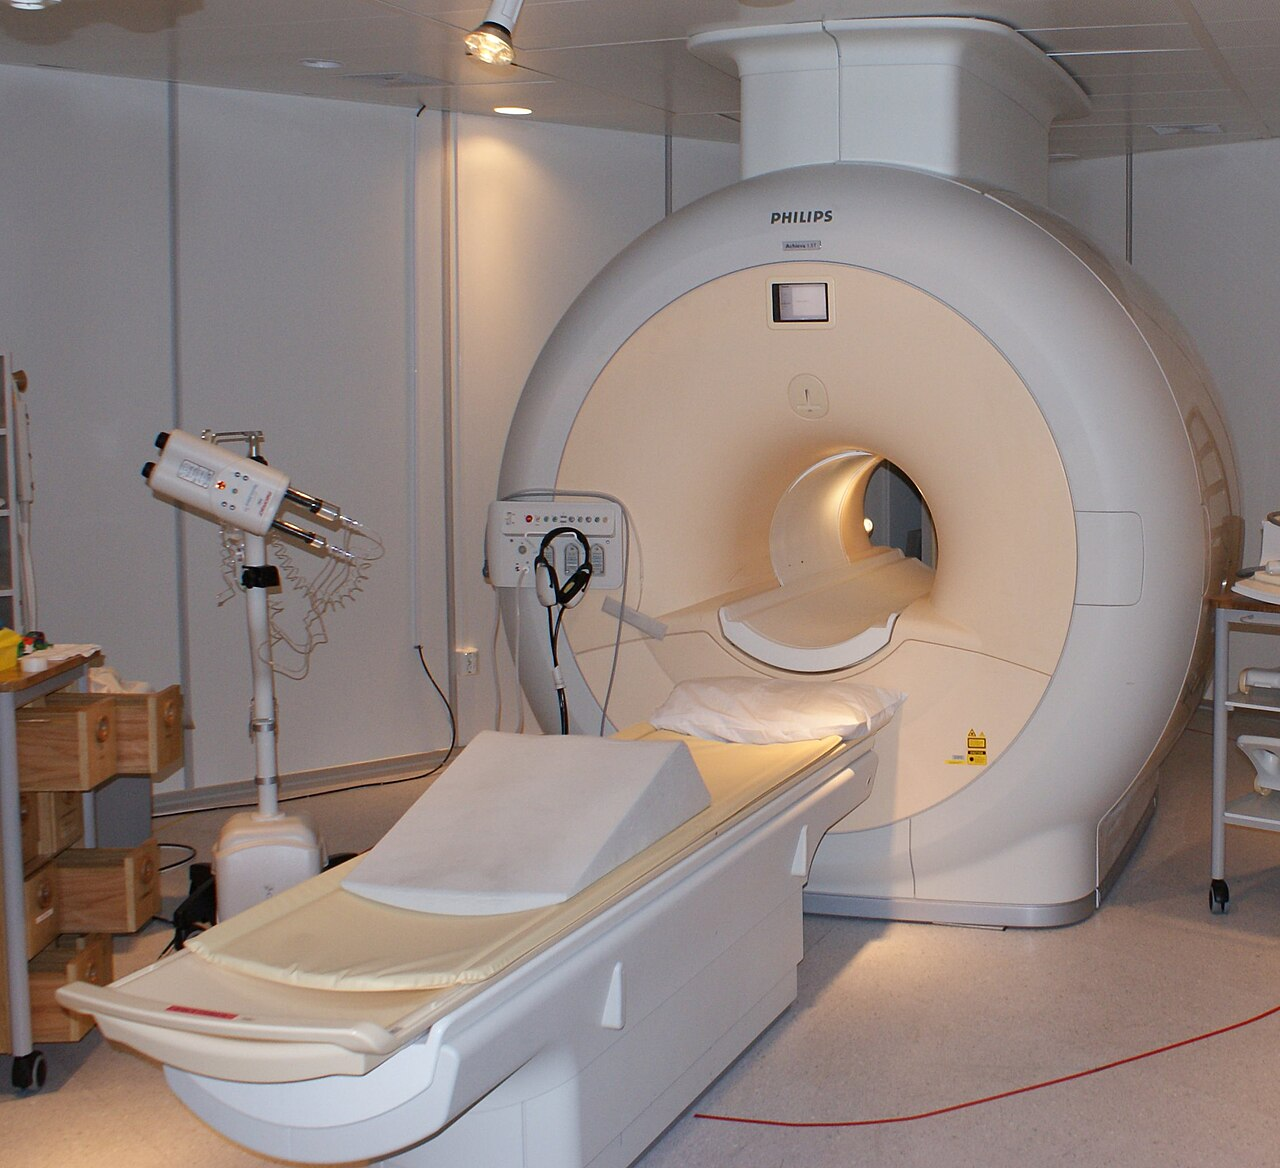
\includegraphics[width=0.50\linewidth]{images/book3/mri-scanner.jpg}

{\small Um aparelho de ressonância magnética: um solenoide supercondutor que mantém \qty{1.5}{T} sobre um paciente --- um megajoule de \omterm{prop:b1:induction:inductor}{energia magnética} num campo com nada dentro. Fotografia: Jan Ainali, CC~BY~3.0.}
\end{omfigure}

\section{A lei de Faraday}

\begin{definition}[Fluxo magnético através de um circuito]\label{def:b1:induction:flux}
\index{fluxo magnético}\index{weber}
Oriente um circuito fechado $\Gamma$ (um sentido de percurso); a sua superfície recebe
a normal $\vect n$ dada pela regra da mão direita. O \emph{fluxo
magnético} através do circuito vale $\Phi = \sum\vect B\cdot\vect n\,\dd S$ sobre
qualquer superfície apoiada em $\Gamma$ (weber, $\qty{1}{Wb} = \qty{1}{T.m^2}$) ---
``qualquer'', porque o fluxo de $\vect B$ através de uma superfície fechada é nulo.
Para um campo uniforme e uma bobina plana de $N$ espiras e área $S$, $\Phi =
NBS\cos\alpha$, sendo $\alpha$ o ângulo entre $\vect B$ e $\vect n$.
\end{definition}

\begin{theorem}[Lei da indução de Faraday]\label{thm:b1:induction:faraday}
\index{lei de Faraday}\index{força eletromotriz (induzida)}\index{lei de Lenz}
Sempre que o fluxo através de um circuito varia, o circuito é sede de
uma \emph{\omterm{def:b1:dc-circuits:sources}{força eletromotriz} induzida}
\[
e = -\frac{\dd\Phi}{\dd t} ,
\]
contada na orientação do circuito, isto é, agindo como uma \omterm{def:b1:dc-circuits:sources}{fonte de
tensão} ideal de fem $e$ nesse sentido; num circuito de resistência $R$
ela faz passar a corrente $i = e/R$. O sinal de menos é a \emph{\omterm{thm:b1:induction:faraday}{lei de Lenz}}:
a corrente induzida circula de modo a se opor à variação de fluxo que a
produz --- o seu próprio campo, e as forças que ela sente, combatem a causa.
\end{theorem}
\admitted

\begin{remark}[Duas faces da mesma lei]\label{rem:b1:induction:twofaces}
\index{indução de Neumann}\index{indução de Lorentz}
O fluxo varia ou porque $\vect B$ varia no tempo através de um
circuito fixo (\emph{\omterm{rem:b1:induction:twofaces}{indução de Neumann}}: transformador, fogão de indução)
ou porque o circuito se move ou se deforma num campo permanente
(\emph{\omterm{rem:b1:induction:twofaces}{indução de Lorentz}}: gerador, alto-falante). No segundo caso
a fem também pode ser calculada diretamente: os portadores de um elemento
condutor $\dd\vect l$ que se move com $\vect v$ sentem a força $q\vect v\wedge
\vect B$, equivalente a um campo elétrico $\vect v\wedge\vect B$, de modo que
$e = \oint(\vect v\wedge\vect B)\cdot\dd\vect l$ --- e isso concorda sempre
com $-\dd\Phi/\dd t$. A \omterm{thm:b1:induction:faraday}{lei de Faraday} cobre os dois casos; o volume do segundo ano
explica por que os dois mecanismos dão uma só fórmula.
\end{remark}

\begin{omfigure}
\begin{tikzpicture}[font=\small, x=1cm, y=1cm, >=Stealth]
  \begin{scope}
    \draw[omThm, very thick, postaction={decorate, decoration={markings, mark=at position 0.25 with {\arrow{>}}, mark=at position 0.75 with {\arrow{>}}}}] (0,0) ellipse (1.4 and 0.5);
    \draw[omDef, thick, ->] (0,0.5) -- (0,1.7) node[right, font=\footnotesize] {$\vect n$};
    \node[omThm, font=\footnotesize] at (1.75,-0.55) {$\Gamma$};
    \foreach \x in {-0.9,-0.3,0.3,0.9} \draw[omProp, ->] (\x,-1.6) -- (\x,1.2);
    \node[omProp, font=\footnotesize] at (1.4,1.05) {$\vect B$};
    \node[font=\footnotesize] at (0,-2.2) {$\Phi = \vect B\cdot\vect n\,S > 0$};
  \end{scope}
  \begin{scope}[xshift=6.2cm]
    \draw[omThm, very thick, postaction={decorate, decoration={markings, mark=at position 0.25 with {\arrow{<}}, mark=at position 0.75 with {\arrow{<}}}}] (0,0) ellipse (1.4 and 0.5);
    \node[omThm, font=\footnotesize] at (1.75,0.6) {$i$};
    % magnet coming down
    \draw[fill=omDef!20, draw=omDef, thick] (-0.4,1.3) rectangle (0.4,2.0); \node[omDef, font=\footnotesize] at (0,1.65) {S};
    \draw[fill=omThm!20, draw=omThm, thick] (-0.4,2.0) rectangle (0.4,2.7); \node[omThm, font=\footnotesize] at (0,2.35) {N};
    \draw[very thick, ->] (0.8,2.6) -- (0.8,1.7) node[right, font=\footnotesize] {$\vect v$};
    \draw[omProp, ->] (0,1.25) -- (0,0.2) node[right, font=\footnotesize, pos=0.6] {$\vect B$ (ímã)};
    \draw[omDef, ->] (-0.6,-0.1) -- (-0.6,0.9) node[left, font=\footnotesize, pos=0.7] {$\vect B_{\text{ind}}$};
    \node[font=\footnotesize] at (0,-2.2) {ímã se aproximando: $i$ o repele};
  \end{scope}
  \begin{scope}[xshift=11.8cm]
    \draw[omThm, very thick] (-1.4,-0.5) rectangle (1.4,0.5);
    \draw[omThm, very thick] (0.5,-0.5) -- (0.5,0.5);
    \draw[omDef, very thick, ->] (0.5,0.5) -- (0.5,-0.5);
    \draw[very thick, ->] (0.6,0.75) -- (1.2,0.75) node[above, font=\footnotesize] {$\vect v$};
    \foreach \x in {-1.1,-0.6,-0.1,0.4,0.9} \node[omProp, font=\scriptsize] at (\x,0.0) {$\odot$};
    \node[omProp, font=\footnotesize] at (1.75,0.0) {$\vect B$};
    \draw[omDef, ->, thick] (0.5,0.0) -- (-0.2,0.0); \node[omDef, font=\footnotesize] at (-0.15,-0.3) {$\vect F$};
    \node[font=\footnotesize] at (0,-2.2) {barra deslizante: o fluxo cresce, $\vect F$ freia};
  \end{scope}
\end{tikzpicture}

{\small Orientação e \omterm{thm:b1:induction:faraday}{lei de Lenz}. À esquerda: a orientação do circuito
fixa $\vect n$ e o sinal de $\Phi$. No meio: um ímã que se aproxima de um
anel aumenta o fluxo; a corrente induzida cria um campo oposto ao
do ímã e o anel o repele. À direita: uma barra que desliza sobre trilhos num
campo dirigido para o leitor; o fluxo do circuito cresce, e a
corrente induzida circula de modo que a \omterm{thm:b1:magnetostatics:laplace}{força de Laplace} sobre a barra se opõe ao
seu movimento.}
\end{omfigure}

\begin{example}[Ordens de grandeza]\label{ex:b1:induction:orders}
Uma bobina de $100$ espiras e \qty{10}{cm^2} no campo da Terra, virada em
\qty{0.1}{s}: $\Delta\Phi = 2 \times 100 \times 10^{-3} \times 5 \times 10^{-5} = \qty{1e-5}{Wb}$,
$e \sim \qty{0.1}{mV}$ --- mensurável com um galvanômetro sensível, do modo como
o campo da Terra foi outrora mapeado. A mesma bobina no entreferro de \qty{1}{T}
de um ímã, retirada em \qty{0.1}{s}: \qty{1}{V}. Uma bobina de transformador de
$1000$ espiras com \qty{1}{T} a \qty{50}{Hz} sobre \qty{10}{cm^2}: $e_{\max} =
1000 \times 10^{-3} \times 314 = \qty{314}{V}$ --- a rede elétrica.
\end{example}

\section{Autoindutância e indutância mútua}

\begin{definition}[Indutância]\label{def:b1:induction:inductance}
\index{autoindutância}\index{henry}\index{indutância mútua}
O fluxo do campo próprio de um circuito através dele mesmo é proporcional à sua
corrente: $\Phi_{\text{próprio}} = Li$, sendo $L > 0$ a sua \emph{autoindutância}
(henry, \unit{H}). O fluxo que o circuito~1 envia através do circuito~2 vale
$\Phi_{1 \to 2} = Mi_1$ e, simetricamente, $\Phi_{2 \to 1} = Mi_2$, sendo $M$
a \emph{indutância mútua} dos dois (com o sinal fixado pelas orientações). O
fluxo total do circuito~1 vale então $\Phi_1 = L_1i_1 + Mi_2$.
\end{definition}

\begin{proposition}[O indutor; o solenoide]\label{prop:b1:induction:inductor}
\index{indutor}\index{energia magnética}\index{densidade de energia do campo magnético}
Um circuito de indutância $L$ percorrido por uma corrente variável é sede
da fem $e = -L\,\dd i/\dd t$: na \omterm{thm:b1:dc-circuits:kirchhoff}{convenção receptor}, essa é a
\omterm{def:b1:dc-circuits:voltage}{tensão} $u = L\,\dd i/\dd t$ do indutor usado desde o
\cref{ch:b1:transient-regimes}. Ele armazena a energia $W = \tfrac12Li^2$.
Um solenoide longo de $n$ espiras por metro, comprimento $\ell$ e seção $S$
tem $L = \mu_0n^2S\ell$; a sua energia armazenada vale $\tfrac12\mu_0n^2I^2S\ell =
\dfrac{B^2}{2\mu_0}\,S\ell$: a \omterm{prop:b1:induction:inductor}{energia magnética} mora no campo, com
densidade $B^2/2\mu_0$, exatamente como a elétrica em $\varepsilon_0E^2/2$.
\end{proposition}

\begin{proof}
Faraday com $\Phi = Li$ e $L$ constante. Energia: a potência recebida pelo
indutor vale $ui = Li\,\dd i/\dd t = \dd(\tfrac12Li^2)/\dd t$. Solenoide:
$B = \mu_0nI$ dentro, fluxo $BS$ através de cada uma das $n\ell$ espiras, logo $\Phi =
\mu_0n^2S\ell I$. A densidade geral fica admitida.
\end{proof}

\begin{example}[Um ímã de ressonância magnética]\label{ex:b1:induction:mri}
\qty{1.5}{T} sobre cerca de um metro cúbico: $B^2/2\mu_0 = 2.25/2.5 \times 10^{-6} =
\qty{0.9}{MJ/m^3}$ --- a energia de uma bateria de carro, guardada no espaço vazio.
Com uma corrente de bobina de \qty{500}{A}, $L = 2W/I^2 = \qty{7}{H}$. Se o
supercondutor de repente se torna resistivo (um \emph{quench}), esse megajoule
vira calor em segundos e evapora centenas de litros de hélio
líquido: a sala do ímã tem um respiro para isso.
\end{example}

\begin{proposition}[O transformador ideal]\label{prop:b1:induction:transformer}
\index{transformador}
Duas bobinas de $N_1$ e $N_2$ espiras enroladas no mesmo núcleo de ferro fechado,
de modo que o mesmo fluxo $\varphi$ atravesse cada espira, obedecem a
\[
\frac{u_2}{u_1} = \frac{N_2}{N_1} , \qquad N_1i_1 + N_2i_2 = 0 \quad\text{(sem perdas em vazio, sem corrente magnetizante)},
\]
de modo que $u_2i_2 = -u_1i_1$: a potência tomada no primário é entregue
no secundário; as tensões variam com a razão de espiras, e as correntes,
inversamente. Só funciona com correntes variáveis.
\end{proposition}

\begin{proof}
$u_1 = N_1\,\dd\varphi/\dd t$ e $u_2 = N_2\,\dd\varphi/\dd t$ (\omterm{thm:b1:dc-circuits:kirchhoff}{convenção receptor}
nas duas, com as orientações escolhidas segundo o fluxo comum): divida.
A relação entre as correntes é a \omterm{thm:b1:magnetostatics:ampere}{lei de Ampère} no núcleo: a sua circulação,
$\mu_0\mu_r$ vezes o total de ampère-espiras, teria de criar o
fluxo; para um núcleo ideal ($\mu_r \to \infty$) isso exige um número de
ampère-espiras que tende a zero, donde $N_1i_1 + N_2i_2 = 0$. Admitido nesta forma.
\end{proof}

\begin{omfigure}
\begin{tikzpicture}[font=\small, x=1cm, y=1cm, >=Stealth]
  % core
  \draw[omExo!60, line width=9pt] (-2,-1.5) rectangle (2,1.5);
  % primary windings
  \foreach \y in {-0.9,-0.6,...,0.9} \draw[omThm, thick] (-2.35,\y) arc[start angle=90, end angle=-90, x radius=0.18, y radius=0.15];
  \foreach \y in {-0.9,-0.6,...,0.9} \draw[omDef, thick] (2.35,\y) arc[start angle=90, end angle=270, x radius=0.18, y radius=0.15];
  \draw[omThm, thick] (-2.35,0.9) -- (-3.2,0.9) node[left, font=\footnotesize] {$u_1$}; \draw[omThm, thick] (-2.35,-1.2) -- (-3.2,-1.2);
  \draw[omDef, thick] (2.35,0.9) -- (3.2,0.9) node[right, font=\footnotesize] {$u_2$}; \draw[omDef, thick] (2.35,-1.2) -- (3.2,-1.2);
  \node[omThm, font=\footnotesize] at (-2.9,0) {$N_1$}; \node[omDef, font=\footnotesize] at (2.9,0) {$N_2$};
  \draw[omProp, thick, dashed, ->] (-1.3,-0.9) -- (-1.3,0.9) -- (1.3,0.9) -- (1.3,-0.9) -- cycle;
  \node[omProp, font=\footnotesize] at (0,0) {fluxo $\varphi$};
  \node[font=\footnotesize] at (0,-2.2) {$u_2/u_1 = N_2/N_1$, \quad $N_1 i_1 = -N_2 i_2$};
  \begin{scope}[xshift=8.6cm]
    \draw[omThm, very thick] (-1.6,0) -- (1.6,0);
    \foreach \x in {-1.3,-0.9,...,1.3} \draw[omThm, thick] (\x,0) arc[start angle=180, end angle=0, x radius=0.2, y radius=0.45];
    \draw[omDef, very thick] (-1.2,-1.1) -- (1.2,-1.1);
    \foreach \x in {-0.9,-0.5,...,0.9} \draw[omDef, thick] (\x,-1.1) arc[start angle=180, end angle=0, x radius=0.2, y radius=0.35];
    \node[omThm, font=\footnotesize] at (-2.1,0.3) {$i_1$, $L_1$}; \node[omDef, font=\footnotesize] at (-1.9,-0.9) {$L_2$};
    \draw[<->, omProp] (0,0.7) -- (0,-0.9) node[midway, right, font=\footnotesize] {$M$};
    \node[font=\footnotesize] at (0,-2.2) {$\Phi_1 = L_1 i_1 + M i_2$};
  \end{scope}
\end{tikzpicture}

{\small À esquerda: um transformador --- duas bobinas num núcleo de ferro fechado
compartilham o mesmo fluxo; as tensões escalam com o número de espiras, e as correntes,
inversamente. À direita: duas bobinas acopladas no ar e a sua \omterm{def:b1:induction:inductance}{indutância
mútua} $M$; o fluxo próprio de uma bobina vale $Li$.}
\end{omfigure}

\section{Condutores em movimento: geradores e motores}

\begin{proposition}[A barra deslizante]\label{prop:b1:induction:rails}
\index{trilhos de Laplace}\index{conversão eletromecânica}
Uma barra de comprimento $\ell$ desliza com velocidade $v$ sobre dois trilhos fechados por uma
resistência $R$, num campo uniforme $B$ normal ao plano. Ela é
sede da fem $e = B\ell v$, faz passar $i = B\ell v/R$ e sente a
\omterm{thm:b1:magnetostatics:laplace}{força de Laplace} $F = B\ell i = B^2\ell^2v/R$ que se \emph{opõe} ao seu movimento.
A potência mecânica gasta para empurrá-la, $Fv$, é igual à \omterm{thm:b1:dc-circuits:kirchhoff}{potência
elétrica} $ei = Ri^2$ dissipada: a barra é um gerador. Alimentada, em vez disso, por uma
fonte $E$, ela é um motor: a corrente $(E - B\ell v)/R$ a empurra
até que a força contraeletromotriz $B\ell v$ equilibre $E$, na velocidade a vazio $E/B\ell$.
\end{proposition}

\begin{proof}
Fluxo $B\ell x$, $e = -B\ell\dot x$ na orientação em que $\vect n$ está
ao longo de $\vect B$; a \omterm{thm:b1:magnetostatics:laplace}{força de Laplace} $i\vect\ell\wedge\vect B$ sobre a corrente
assim orientada aponta contra $\vect v$ (\cref{thm:b1:induction:faraday},
Lenz). Multiplique a equação elétrica $e = Ri$ por $i$ e a
mecânica por $v$: $Fv = B\ell iv = ei$. A potência eletromecânica
$ei$ e a potência de Laplace $-Fv$ são sempre opostas --- é a lei
da conversão.
\end{proof}

\begin{proposition}[A espira girante: o alternador]\label{prop:b1:induction:alternator}
\index{alternador}
Uma bobina de $N$ espiras e área $S$ que gira com \omterm{cor:b1:point-kinematics:circular}{velocidade angular} $\omega$ em torno de um eixo
perpendicular a um $B$ uniforme tem $\Phi = NBS\cos\omega t$ e
\[
e = NBS\omega\sin\omega t :
\]
uma fem senoidal de \omterm{def:b1:wave-propagation:signal}{amplitude} $NBS\omega$ e frequência igual à de rotação.
Numa resistência $R$ ela entrega a \omterm{thm:b1:sinusoidal-impedance:power}{potência média} $(NBS\omega)^2/2R$,
fornecida pelo \omterm{def:b1:angular-momentum:moment}{torque} que a mantém girando contra o binário de Laplace
$-\vect m\wedge\vect B$ da sua própria corrente.
\end{proposition}

\begin{proof}
Derive o fluxo; $\langle\sin^2\rangle = \tfrac12$. O binário é o do
\cref{thm:b1:magnetostatics:dipoleinfield} com $m = Ni S$; a sua \omterm{thm:b1:sinusoidal-impedance:power}{potência
média} $\langle\Gamma\omega\rangle$ é igual a $\langle ei\rangle$ pelo mesmo
cálculo feito para a barra.
\end{proof}

\begin{omfigure}
\begin{tikzpicture}[font=\small, x=1cm, y=1cm, >=Stealth]
  \begin{scope}
    \draw[omThm, very thick] (-1.8,-1.0) -- (1.8,-1.0); \draw[omThm, very thick] (-1.8,1.0) -- (1.8,1.0);
    \draw[omThm, very thick] (-1.8,-1.0) -- (-1.8,1.0);
    \draw[omDef, very thick] (0.8,-1.0) -- (0.8,1.0);
    \draw[omDef, very thick, ->] (0.8,-0.2) -- (0.8,0.3) node[right, font=\footnotesize] {$i$};
    \draw[omProp, thick, ->] (0.8,0) -- (0.05,0) node[above, font=\footnotesize, pos=0.5] {$\vect F$};
    \draw[very thick, ->] (1.0,1.25) -- (1.7,1.25) node[right, font=\footnotesize] {$\vect v$};
    \foreach \x in {-1.4,-0.9,-0.4,0.1,1.3} \foreach \y in {-0.5,0.5} \node[omProp, font=\scriptsize] at (\x,\y) {$\odot$};
    \draw[fill=white] (-1.95,-0.35) rectangle (-1.65,0.35); \node[font=\footnotesize] at (-2.45,0) {$R$};
    \node[font=\footnotesize] at (0,-1.6) {$e = B\ell v$, \; $F = B^2\ell^2 v/R$};
  \end{scope}
  \begin{scope}[xshift=6.5cm]
    \draw[omThm, very thick, rotate=30] (-1.2,-0.6) rectangle (1.2,0.6);
    \draw[dashed] (0,-1.6) -- (0,1.6); \node[font=\footnotesize] at (0,1.85) {eixo};
    \foreach \y in {-1.2,-0.6,0,0.6,1.2} \draw[omProp, ->] (-2.2,\y) -- (2.2,\y);
    \node[omProp, font=\footnotesize] at (2.0,1.45) {$\vect B$};
    \draw[->, very thick] (0,0) -- (120:1.0) node[above left, font=\footnotesize] {$\vect n$};
    \draw (0.6,0) arc[start angle=0, end angle=120, radius=0.6] node[midway, above right, font=\footnotesize] {$\omega t$};
    \node[font=\footnotesize] at (0,-2.0) {$\Phi = NBS\cos\omega t$, \; $e = NBS\omega\sin\omega t$};
  \end{scope}
\end{tikzpicture}\hfill
\begin{tikzpicture}
\begin{axis}[omaxis, axis x line=middle, axis y line=left, width=4.3cm, height=3.8cm,
    xlabel={$t$}, ylabel={$e$}, xmin=0, xmax=6.6, ymin=-1.3, ymax=1.3, xtick=\empty, ytick=\empty, samples=80,
    xlabel style={at={(axis description cs:1.0,0.55)}, anchor=west}]
  \addplot[omDef, thick, domain=0:6.28] {sin(deg(x))};
\end{axis}
\end{tikzpicture}

{\small À esquerda: a barra deslizante como gerador --- fem $B\ell v$, corrente
através de $R$, \omterm{thm:b1:magnetostatics:laplace}{força de Laplace} freando a barra; a potência de quem empurra é o
calor do \omterm{def:b1:dc-circuits:resistor}{resistor}. No meio e à direita: a bobina girante de um alternador
e a sua fem senoidal.}
\end{omfigure}

\begin{example}[Correntes de Foucault]\label{ex:b1:induction:eddy}
\index{correntes de Foucault}
Um condutor maciço que se move num campo não uniforme, ou que fica num campo
variável, é atravessado por fluxo variável ao longo de incontáveis caminhos fechados:
as \emph{\omterm{ex:b1:induction:eddy}{correntes de Foucault}} circulam nele, aquecendo-o e --- por Lenz ---
freando-o. Um ímã largado dentro de um tubo de cobre desce devagar; os
freios de caminhões e de montanhas-russas usam isso (sem contato, sem desgaste, sem
falha de freio --- mas sem frenagem em repouso); o fogão de indução aquece
a panela pelas mesmas correntes, a \qty{25}{kHz}; e os núcleos de transformador são
laminados justamente para cortá-las.
\end{example}

\section{O alto-falante: um sistema acoplado}

\begin{proposition}[Acoplamento eletromecânico de uma bobina num campo radial]\label{prop:b1:induction:loudspeaker}
\index{alto-falante}\index{microfone}
Uma bobina de comprimento total de fio $\ell$ fica num campo radial $B$, de modo que
cada elemento de fio é perpendicular a $\vect B$; ela se move ao longo do seu
eixo com velocidade $v$ e conduz $i$. Ela sente então a \omterm{thm:b1:magnetostatics:laplace}{força de Laplace} axial
$F = B\ell i$ e é sede da força contraeletromotriz $e = -B\ell v$ (na \omterm{thm:b1:dc-circuits:kirchhoff}{convenção
receptor}: uma \omterm{def:b1:dc-circuits:voltage}{tensão} $B\ell v$). Com uma massa $m$, uma suspensão de
rigidez $k$ e um amortecimento mecânico $h$, alimentada por uma \omterm{def:b1:dc-circuits:voltage}{tensão} $u$ através
da resistência $R$ e da indutância $L$ da bobina:
\[
u = Ri + L\frac{\dd i}{\dd t} + B\ell v , \qquad
m\frac{\dd v}{\dd t} = -kx - hv + B\ell i .
\]
Multiplicando por $i$ e por $v$ e somando: a \omterm{thm:b1:dc-circuits:kirchhoff}{potência elétrica} $ui$
é igual à perda Joule $Ri^2$ mais o crescimento das energias armazenadas
$\tfrac12Li^2 + \tfrac12mv^2 + \tfrac12kx^2$ mais a perda mecânica
$hv^2$ (que inclui o som): o termo de conversão $B\ell iv$ se cancela
entre as duas equações. Funcionando ao contrário (movimento imposto, $u$ lido), o
mesmo dispositivo é um \emph{microfone} dinâmico.
\end{proposition}

\begin{proof}
\omterm{thm:b1:magnetostatics:laplace}{Força de Laplace} sobre cada elemento $i\,\dd\vect l\wedge\vect B$, todas axiais e
de mesmo sinal; fem por $(\vect v\wedge\vect B)\cdot\dd\vect l$ somado
sobre o fio. O balanço de energia é a soma das duas equações
multiplicadas como se disse.
\end{proof}

\begin{omfigure}
\begin{tikzpicture}[font=\small, x=1cm, y=1cm, >=Stealth]
  % magnet structure (cross-section)
  \draw[fill=omExo!30, draw=omExo, thick] (-3.0,-1.2) rectangle (-0.6,1.2);
  \draw[fill=omExo!30, draw=omExo, thick] (-0.6,-0.35) rectangle (1.6,0.35);
  \draw[fill=omExo!30, draw=omExo, thick] (-0.6,0.85) rectangle (1.6,1.2);
  \draw[fill=omExo!30, draw=omExo, thick] (-0.6,-1.2) rectangle (1.6,-0.85);
  \node[omExo, font=\footnotesize] at (-1.8,0) {ímã};
  % coil in the gaps
  \foreach \x in {0.9,1.05,1.2,1.35} {\fill[omThm] (\x,0.6) circle (1.6pt); \fill[omThm] (\x,-0.6) circle (1.6pt);}
  \node[omThm, font=\footnotesize] at (1.1,1.55) {bobina móvel};
  % radial field arrows in the gaps
  \foreach \x in {0.3,0.55} {\draw[omProp, ->] (\x,0.4) -- (\x,0.8); \draw[omProp, ->] (\x,-0.4) -- (\x,-0.8);}
  \node[omProp, font=\footnotesize] at (-0.2,0.6) {$\vect B$};
  % cone
  \draw[thick] (1.6,0.6) -- (3.4,2.2); \draw[thick] (1.6,-0.6) -- (3.4,-2.2);
  \draw[thick] (1.6,0.6) -- (1.6,-0.6);
  \node[font=\footnotesize] at (2.9,-0.95) {cone, $m$};
  \draw[thick, decorate, decoration={coil, aspect=0.6, segment length=3pt, amplitude=2pt}] (3.4,2.2) -- (3.4,2.9); \draw[thick] (3.0,2.9) -- (3.8,2.9);
  \draw[thick, decorate, decoration={coil, aspect=0.6, segment length=3pt, amplitude=2pt}] (3.4,-2.2) -- (3.4,-2.9); \draw[thick] (3.0,-2.9) -- (3.8,-2.9);
  \node[font=\footnotesize] at (3.4,3.25) {suspensão $k$, $h$};
  \draw[omDef, very thick, ->] (1.6,0) -- (2.6,0);
  \node[omDef, font=\footnotesize, anchor=south west] at (1.75,0.08) {$F = B\ell i$};
  \draw[very thick, ->] (4.6,0.5) -- (5.6,0.5) node[right, font=\footnotesize] {$v$};
  \node[font=\footnotesize] at (5.3,-1.7) {$u = Ri + L\frac{\dd i}{\dd t} + B\ell v$};
\end{tikzpicture}

{\small Um alto-falante de bobina móvel em corte: a bobina fica no
entreferro anular de um ímã onde o campo é radial, de modo que uma
corrente dá uma força axial qualquer que seja a posição; o cone que ela move
é preso por uma suspensão rígida e amortecida; o movimento da bobina injeta uma
força contraeletromotriz $B\ell v$ no circuito elétrico.}
\end{omfigure}

\begin{remark}[Por que o acoplamento amortece]\label{rem:b1:induction:damping}
Em baixa frequência ($L\omega \ll R$), $i \approx (u - B\ell v)/R$ e a força vale
$B\ell u/R - (B^2\ell^2/R)\,v$: o circuito elétrico acrescenta o amortecimento
$B^2\ell^2/R$ ao mecânico. Um alto-falante ligado a um
amplificador (de baixa resistência de saída) fica bastante amortecido --- o seu cone para
quando o sinal para --- e o mesmo acoplamento é o que permite ao
microfone tirar energia do som (\cref{pb:b1:induction:1}).
\end{remark}

\section{Exercícios}

\begin{exercise}[$\star$]\label{exo:b1:induction:1}
Uma bobina de $100$ espiras e \qty{10}{cm^2} num campo uniforme de \qty{0.20}{T} a
\qty{30}{\degree} da sua normal. Fluxo; fem média se o campo for desligado
em \qty{10}{ms}; e em \qty{1}{ms}; sentido da corrente induzida
em relação ao campo (Lenz).
\end{exercise}

\begin{exercise}[$\star$]\label{exo:b1:induction:2}
Uma barra de \qty{20}{cm} desliza a \qty{2.0}{m/s} sobre trilhos fechados por
\qty{0.10}{\ohm}, em \qty{0.50}{T}. Fem, corrente, \omterm{thm:b1:magnetostatics:laplace}{força de Laplace}, força que
quem empurra tem de aplicar, potência mecânica, \omterm{thm:b1:dc-circuits:kirchhoff}{potência elétrica}.
\end{exercise}

\begin{exercise}[$\star$]\label{exo:b1:induction:3}
Solenoide de \qty{1000}{espiras/m}, comprimento \qty{20}{cm}, seção \qty{4.0}{cm^2}:
indutância; energia a \qty{5.0}{A}; \omterm{def:b1:transient-regimes:firstorder}{constante de tempo} com uma resistência de
\qty{1.0}{\ohm}; campo dentro e densidade de energia, para verificar $B^2/2\mu_0$.
\end{exercise}

\begin{exercise}[$\star$]\label{exo:b1:induction:4}
Um transformador de \qty{230}{V} para \qty{12}{V}: razão de espiras; espiras do
primário para um secundário de $50$ espiras; corrente do primário quando o secundário
entrega \qty{2.0}{A}. Por que ele não funciona com uma bateria de carro?
\end{exercise}

\begin{exercise}[$\star\star$]\label{exo:b1:induction:5}
\omterm{thm:b1:induction:faraday}{Lei de Lenz}: dê o sentido da corrente induzida e a direção da
força em cada caso --- (a) um polo norte se aproxima de um anel ao longo
do seu eixo; (b) um anel está num campo que cresce; (c) um anel é largado
sobre um ímã; (d) um ímã cai dentro de um tubo longo de cobre. Para (d),
explique pela energia por que ele cai com velocidade constante e pequena.
\end{exercise}

\begin{exercise}[$\star\star$]\label{exo:b1:induction:6}
Alternador: $N = 200$, $S = \qty{20}{cm^2}$, $B = \qty{0.10}{T}$, \qty{50}{Hz}.
Fem de pico e eficaz; corrente de pico e \omterm{def:b1:angular-momentum:moment}{torque} de pico em \qty{10}{\ohm}; \omterm{thm:b1:dc-circuits:kirchhoff}{potência
elétrica} média; compare com a potência mecânica média e com o
\omterm{def:b1:angular-momentum:moment}{torque} instantâneo no momento em que a fem se anula.
\end{exercise}

\begin{exercise}[$\star\star$]\label{exo:b1:induction:7}
\emph{Freio magnético.} Uma espira quadrada de lado $a = \qty{10}{cm}$ e
resistência $R = \qty{1.0}{m\ohm}$, de massa \qty{1.0}{kg}, sai de uma região de
campo uniforme $B = \qty{1.0}{T}$ com velocidade $v$ (um lado ainda dentro do
campo). Fem, corrente, força de frenagem; equação do movimento e \omterm{def:b1:transient-regimes:firstorder}{constante
de tempo}; distância percorrida antes de parar a partir de \qty{1.0}{m/s}; para onde
foi a \omterm{thm:b1:work-and-energy:ke}{energia cinética}?
\end{exercise}

\begin{exercise}[$\star\star$]\label{exo:b1:induction:8}
Uma pequena bobina ($N_2 = 50$ espiras, seção \qty{2.0}{cm^2}) fica dentro de um
solenoide longo ($n_1 = \qty{2000}{m^{-1}}$), com os eixos alinhados. \omterm{def:b1:induction:inductance}{Indutância
mútua}; fem na bobina quando a corrente do solenoide cresce a
\qty{100}{A/s}, e quando ela vale $\qty{1.0}{A}$ a \qty{10}{kHz}. $M$
depende de qual bobina conduz a corrente?
\end{exercise}

\begin{exercise}[$\star\star$]\label{exo:b1:induction:9}
Energia num campo: $B = \qty{1.5}{T}$ sobre \qty{1.0}{m^3}, como num ímã de
ressonância magnética. Energia; indutância para $I = \qty{500}{A}$; altura a que essa
energia elevaria um carro de \qty{1}{t}; volume de hélio líquido que ela evapora
num quench (\qty{2.6}{kJ} por litro). Energia do campo da Terra
(\qty{5e-5}{T}) numa sala de \qty{50}{m^3}.
\end{exercise}

\begin{exercise}[$\star\star\star$]\label{exo:b1:induction:10}
\emph{Trilhos como motor.} A barra do \cref{exo:b1:induction:2} (massa $m$,
sem atrito) é ligada a uma fonte $E$ através da resistência $R$.
(a) Equações elétrica e mecânica; mostre que $m\,\dd v/\dd t = B\ell(E -
B\ell v)/R$. (b) \omterm{prop:b1:newton-dynamics:terminal}{Velocidade limite} e \omterm{def:b1:transient-regimes:firstorder}{constante de tempo}. (c) Balanço de potência:
potência da fonte $=$ Joule $+$ mecânica; \omterm{def:b1:heat-engines:efficiency}{rendimento} em função de
$v$. (d) Números: $E = \qty{2.0}{V}$, $m = \qty{50}{g}$, o resto como no
\cref{exo:b1:induction:2}. (e) Um canhão eletromagnético acelera um projétil de \qty{10}{g}
com \qty{1}{MA} ao longo de \qty{5}{m} em \qty{1}{T}: velocidade de saída
(\omterm{def:b1:units-dimensions:oom}{ordem de grandeza}).
\end{exercise}

\begin{exercise}[$\star\star\star$]\label{exo:b1:induction:11}
\emph{O disco de Faraday.} Um disco de cobre de raio $R$ gira com \omterm{cor:b1:point-kinematics:circular}{velocidade angular} $\omega$
em torno do seu eixo num $B$ uniforme paralelo ao eixo; escovas tocam o centro
e a borda. (a) Fem entre o centro e a borda somando $(\vect v\wedge
\vect B)\cdot\dd\vect l$ ao longo de um raio: $e = \tfrac12B\omega R^2$. (b) Números:
$R = \qty{10}{cm}$, \qty{3000}{rpm}, \qty{1.0}{T}. (c) Por que ele é uma máquina
de baixa \omterm{def:b1:dc-circuits:voltage}{tensão} e alta corrente; corrente em \qty{1}{m\ohm} e o
\omterm{def:b1:angular-momentum:moment}{torque} de frenagem. (d) Recupere $e$ pela \omterm{thm:b1:induction:faraday}{lei de Faraday} aplicada ao
circuito escova--raio--borda--escova: que fluxo varia?
\end{exercise}

\begin{exercise}[$\star\star\star$]\label{exo:b1:induction:12}
\emph{Fogão de indução.} A bobina sob o vidro conduz $i_1 =
I_1\cos\omega t$ com $I_1 = \qty{30}{A}$ a \qty{25}{kHz}; o fundo da panela
age como uma única espira de resistência $R_p = \qty{10}{m\ohm}$, acoplada por
$M = \qty{1.0}{\micro H}$ (desprezada a indutância da espira da panela). (a) Fem
induzida na panela, valor de pico. (b) Corrente e \omterm{thm:b1:sinusoidal-impedance:power}{potência média} dissipada
na panela. (c) Por que uma frequência alta, e por que o calor aparece na
panela e não no vidro? (d) A corrente da panela reage sobre a bobina:
fem que ela induz ali (de pico) e potência extra que o gerador tem de
fornecer --- verifique que ela é igual à de (b).
\end{exercise}

\begin{omfigure}
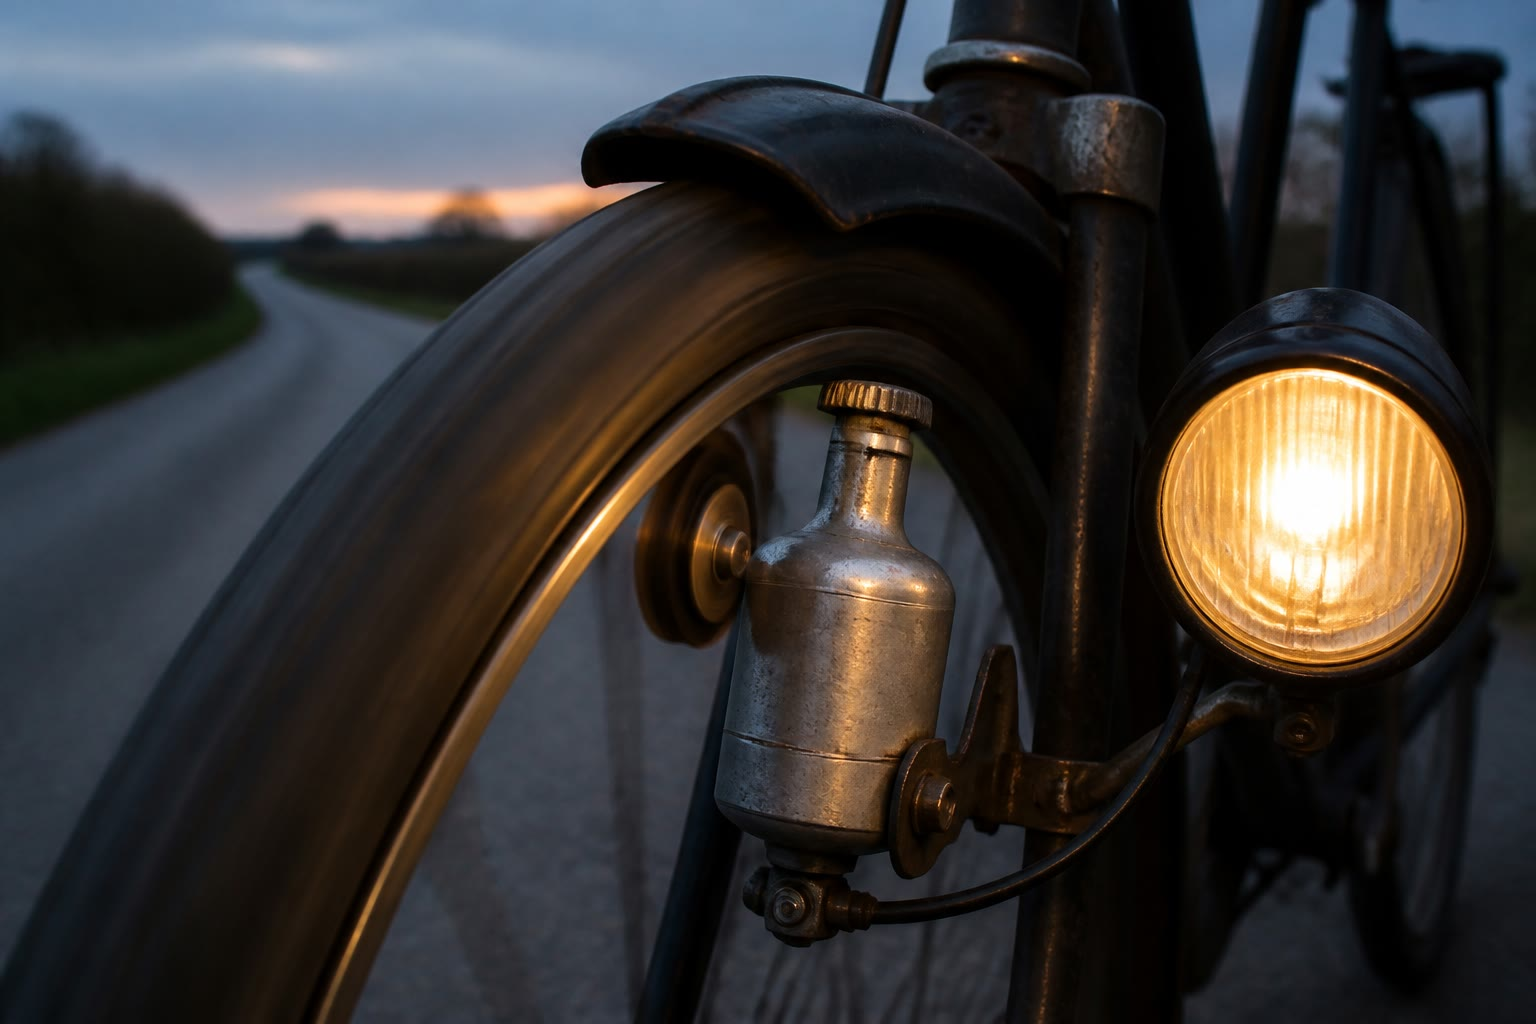
\includegraphics[width=0.58\linewidth]{images/book3/ai/b3-29-bicycle-dynamo.jpg}

{\small Um dínamo de garrafa: a roda gira um ímã dentro de uma bobina, o fluxo através da bobina muda, e a lâmpada acende --- a \omterm{thm:b1:induction:faraday}{lei de Faraday} numa bicicleta.}
\end{omfigure}

\section{Problema: o dínamo de bicicleta e o alto-falante}

\begin{problem}[{Problema de fim de semana --- dois conversores eletromecânicos
desmontados: um dínamo que se regula sozinho e um alto-falante cujo
amplificador é também o seu freio}]
\label{pb:b1:induction:1}

\medskip
\noindent\textbf{Parte I --- O dínamo de bicicleta.}
Uma bobina de $N = 300$ espiras e área $S = \qty{3.0}{cm^2}$ gira num
campo uniforme $B = \qty{0.30}{T}$; o seu eixo leva uma roldana de raio
$r = \qty{1.0}{cm}$ pressionada contra o pneu, de modo que a bobina gira com
$\omega = v/r$ para uma velocidade $v$ da bicicleta. Resistência da bobina $r_c = \qty{4.0}{\ohm}$,
indutância $L = \qty{20}{mH}$; a lâmpada é uma resistência $R = \qty{12}{\ohm}$.
\begin{enumerate}
  \item Fluxo através da bobina e fem induzida em função do tempo;
        \omterm{def:b1:wave-propagation:signal}{amplitude} e frequência a $v = \qty{18}{km/h}$.
  \item Desprezando $L$ de início: corrente eficaz e potência na lâmpada a
        \qty{18}{km/h}; uma lâmpada de ``\qty{6}{V}, \qty{3}{W}'' fica confortável?
  \item Potência mecânica média que o ciclista fornece ao dínamo e a
        força correspondente sobre o pneu (compare com o atrito de
        rolamento, cerca de \qty{2}{N}).
  \item Explique pela \omterm{thm:b1:induction:faraday}{lei de Lenz} por que o dínamo resiste, e por que uma lâmpada
        que acende ``de graça'' não contradiz a conservação da energia.
  \item Inclua agora $L$: \omterm{def:b1:sinusoidal-impedance:impedance}{impedância} complexa do circuito; mostre que
        a \omterm{def:b1:wave-propagation:signal}{amplitude} da corrente vale $I = NBS\omega/\sqrt{(R + r_c)^2 + L^2\omega^2}$
        e que ela satura em alta velocidade; o seu limite e a
        velocidade em que ela atinge $70\%$ do limite.
  \item Sem a indutância, o que a lâmpada receberia a
        \qty{54}{km/h} numa descida? E com ela?
  \item Corrente e potência da lâmpada a \qty{9}{km/h} e a \qty{36}{km/h}; comente
        a autorregulação.
  \item Os dínamos reais giram um ímã dentro de uma bobina fixa. A
        análise muda? Que problema prático isso elimina?
  \item O que a lâmpada faz quando a bicicleta para num sinal vermelho,
        e como as lanternas modernas resolvem isso?
\end{enumerate}

\medskip
\noindent\textbf{Parte II --- O alto-falante.}
Bobina móvel: comprimento de fio $\ell = \qty{5.0}{m}$ num campo radial $B =
\qty{1.0}{T}$, resistência $R = \qty{8.0}{\ohm}$, indutância $L = \qty{0.50}{mH}$;
massa móvel (bobina e cone) $m = \qty{10}{g}$; rigidez da suspensão
$k = \qty{1000}{N/m}$, amortecimento mecânico $h = \qty{1.0}{N.s/m}$. Regime
senoidal, \omterm{def:b1:sinusoidal-impedance:complex}{amplitudes complexas}.
\begin{enumerate}[resume]
  \item Força sobre a bobina para uma corrente $i$; força contraeletromotriz para uma velocidade $v$
        (deduza as duas, com os sinais).
  \item Escreva as equações elétrica e mecânica.
  \item Elimine $i$ e mostre que
        $\underline v = \dfrac{B\ell\,\underline u}{(R + jL\omega)(jm\omega + h + k/j\omega) + B^2\ell^2}$.
  \item Nas frequências em que $L\omega \ll R$, mostre que o acoplamento age
        como um amortecimento mecânico suplementar $B^2\ell^2/R$; valor; frequência de
        ressonância do cone e o seu \omterm{def:b1:transient-regimes:secondorder}{fator de qualidade} com e sem
        o amortecimento elétrico.
  \item O amplificador entrega $i$ de \omterm{def:b1:wave-propagation:signal}{amplitude} \qty{1.0}{A} a \qty{1}{kHz}:
        \omterm{def:b1:wave-propagation:signal}{amplitudes} de força, aceleração, deslocamento e velocidade do
        cone (regime controlado pela massa); \omterm{def:b1:wave-propagation:signal}{amplitude} da força contraeletromotriz comparada com
        $Ri$.
  \item A mesma corrente na frequência de ressonância: \omterm{def:b1:wave-propagation:signal}{amplitude} da velocidade
        (regime controlado pelo amortecimento) e força contraeletromotriz; comente.
  \item \omterm{thm:b1:dc-circuits:kirchhoff}{Potência elétrica} a \qty{1}{kHz}; potência mecânica dissipada em
        $h$ (tomada como o som e as perdas da suspensão); \omterm{def:b1:heat-engines:efficiency}{rendimento}.
  \item Por que o fato de a pressão sonora ser proporcional à aceleração
        do cone (admita-o) é a razão de um cone controlado pela massa dar uma
        resposta plana acima da ressonância?
  \item Por que o campo tem de ser radial, e por que um tweeter é pequeno?
  \item Esboce o módulo da \omterm{def:b1:sinusoidal-impedance:impedance}{impedância} $\underline u/\underline i$ vista
        pelo amplificador de \qty{10}{Hz} a \qty{10}{kHz}: valor em baixa
        frequência, na ressonância (use a velocidade controlada pelo amortecimento)
        e a \qty{10}{kHz}.
\end{enumerate}

\medskip
\noindent\textbf{Parte III --- Ao contrário, e as contas.}
\begin{enumerate}[resume]
  \item O mesmo dispositivo como microfone: um som move o cone a
        $v = \qty{1.0}{mm/s}$; \omterm{def:b1:dc-circuits:voltage}{tensão} em circuito aberto.
  \item Carregado por $R_L = \qty{600}{\ohm}$: corrente e força de frenagem
        sobre o cone; mostre que o microfone tira potência do som
        por um amortecimento efetivo $B^2\ell^2/(R + R_L)$.
  \item A bobina é enrolada sobre um cilindro de alumínio (o carretel), uma
        espira fechada de comprimento \qty{0.10}{m} e resistência \qty{1.0}{m\ohm}:
        amortecimento que ele acrescenta; por que os carretéis são fendidos.
  \item Bata no cone de um alto-falante cujos terminais estão em aberto e depois
        no de um cujos terminais estão em curto: qual dos dois soa por mais tempo,
        e por quê?
  \item Escreva o balanço de energia do alto-falante ao longo de um período em
        \omterm{def:b1:transient-regimes:firstorder}{regime permanente}, nomeando cada termo.
  \item Resuma: para cada dispositivo, a lei usada e os dois números
        que vale a pena guardar.
\end{enumerate}
\end{problem}
